%!TEX root = report.tex
\newpage
\section{Experimental Setup}

% Camera
\subsection{Camera Setup}

\paragraph{Hardware} The camera is made of a Raspberry Pi 2 Model B with the corresponding Raspi-Camera module. 
The Operating System loaded on the Raspberry Pi is the common Raspian WHEEZY system with some costumizations and two scripts that are ran on startup. 

The camera has the following key parameters \cite{RaspiDoc}
\begin{itemize}
    \item Pixel Count: 2592 $\times$ 1944 (chosen resolution: 1280 $\times$ 720)
    \item Pixel size 1.4 x 1.4 $\mu m$
    \item Focal width and length: $f=3.6mm$
\end{itemize}

\begin{figure}[H]
    \centering
    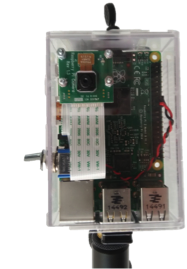
\includegraphics[width=0.3\linewidth]{files/RaspiCam.png}
    \caption{Raspberry Pi with camera module used for visual localization.}
    \label{fig:camera}
\end{figure}


\paragraph{Webcam setup} In order to connect to the local network on startup, a few lines of code need to be added in the Rasperry Pi's \texttt{/etc/network/interfaces} 

\begin{center}
\begin{minipage}{0.9\linewidth}
    \begin{lstinputlisting}[caption=\texttt{/etc/network/interfaces}., label=interfaces, frame=none]
        {files/interfaces}
\end{lstinputlisting}
\end{minipage}
\end{center}

The camera module comes with its own library for taking single images ($raspistill$) or videos ($raspivid$).
The following lines of code are added in a file \texttt{$\sim$/start\_camera.sh} in order to take pictures at regular intervals and serve them on a local server. 
\begin{center}
\begin{minipage}{0.9\linewidth}
\begin{lstinputlisting}[caption=\texttt{$\sim$/start\_camera.sh}., label=startcamera, frame=none]
    {files/start_camera}
\end{lstinputlisting}
\end{minipage}
\end{center}

Line 6 makes the camera take a picture of resolution $w \times h = 1280 \times 720$ of quality $q=50\%$ (100\% would mean no compression at all), at a time interval of $tl = 100 \text{ ms}$ until the time $t = 2'147'483'647 \text{ ms} = 24 \text{ d} 19 \text{ h}$ is reached, which is the maximum for a 32-bit signed integer.
Other parameters like the exposure, set to backlight, and the metering mode can be set. 
With these settings, the resulting picture size is of about $N_{pic}=455\text{ kB}$, which, compared to a size of around $N_{pic}=533 \text{ kB}$ for 100\% quality does not represents a relevant decrease in size. 
\begin{figure}[htb]
    \centering
    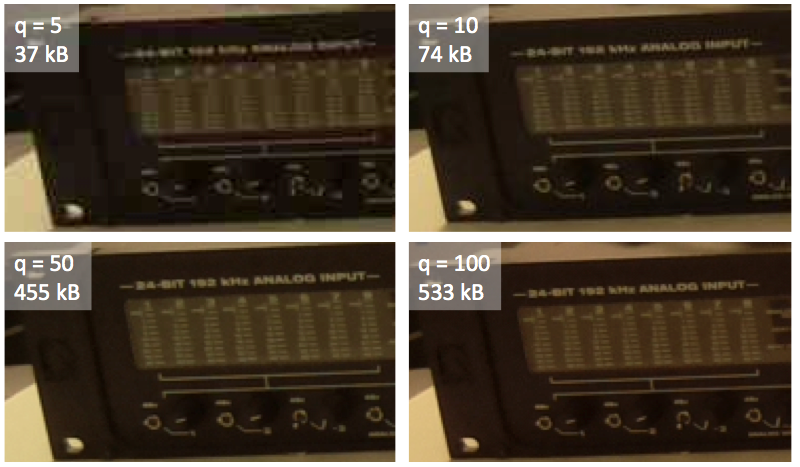
\includegraphics[width=.8\linewidth]{files/quality.png}
    \caption{Quality vs. image size considerations}
    \label{fig:quality}
\end{figure}
The way the image compression is implemented, there is nearly no difference in size down to a quality of around 20\% and the loss in quality is negligible (see Figure \ref{fig:quality}).
The size obtained with $q=50\%$ is too large for the chosen Router that has a capacity of about 150 Mbps, considering that in the worst case, the images from the four cameras are required simultaneously. 
Therefore the compression measure is set down to $q=10\%$, which is a good trade off between image quality and size (see Figure \ref{fig:quality}). 
Indeed, this quality is said to be equivalent to 85\% for most image processing applications by Raspberry Pi users. %TODO add citation?
Finally the thumbnail, which is a bitmap that also takes up unnecessary storage space, is deleted to obtain the final image size of $N_{pic}=80 \text{ kB}$. This is an acceptable size since we have
\begin{equation}
    S_{network} = 150 \text{ Mbps} = 18.75 \text{ MB/s} \geq \frac{N_{pic}}{tl}  = \frac{80/1024 \text{ MB}}{0.1\text{s}}= 0.78 \text{ MB/s}.
\end{equation}

This leads to a reasonable security margin, which is desirbale since measurements show that the declared maximum capacity is largely overestimated. %indicating a capacity of only 1.5-1.7 MB/s.

The pictures are saved as \texttt{/tmp/stream/pic.jpg}, a folder with all permissions, created for this purpose only (Lines 4 and 5).
This is where the current picture will be found by the $mjpg-streamer$ module which serves it on a webpage. 
The $mjpg-streamer$ is a Linux-UVC streaming application which streams JPGs from webcams, filesystems or other input plugins as \textit{M-JPEG}, which is a common video compression format, via HTTP to webbrowsers.


\paragraph{Button}

A button is added to the camera such that it can be restarted or turned off without connecting to the camera via ssh. This allows the Raspberry to be turned off correctly even when the network has not be set up properly or the ethernet is not working.
The button is a pull-down resistor, thus the signal at the output goes from 0 to 1 when the button is pressed. 
An interrupt is triggered when the button is pressed in which it registers during six seconds whether the button is still pressed at a rate of 1s. For robustness, a total of 3 signals is sufficient for the system to shut down. If less than 3 signals are registered during the 6 seconds, the system reboots. 
The \textit{python} script implementing this is shown in Listing \ref{switchoff}.

\begin{center}
\begin{minipage}{0.9\linewidth}
    \begin{lstinputlisting}[caption=\texttt{$\sim$\/switchoff.py}, label=switchoff, language=Python, frame=none]{files/switchoff.py}
\end{lstinputlisting}
\end{minipage}
\end{center}


Both scripts above need to be started on startup of the camera. Therefore, the following lines are put in the file \texttt{/etc/rc.local}.
\begin{center}
\begin{minipage}{0.9\linewidth}
    \begin{lstlisting}[caption=\texttt{/etc/rc.local}, label=local, frame=none]
#Auto start camera
sudo /home/pi/start_camera.sh &
#Auto start shutdown
sudo python /home/pi/switchoff.py &
\end{lstlisting}
\end{minipage}
\end{center}

\subsection{Audio Setup}
The tools used for the audio recording are two wireless audio transmitters with their corresponding 
receivers (\textit{Line 6 Relay G50}, see Figure \ref{fig:audio}) 
with the following key specifications.

\begin{itemize}
    \item Frequency range 10 Hz - 20 kHz
    \item Distance range ca. 61 m (200 ft)
    \item Broadcast in 2.4 GHz band
\end{itemize}

The transmitters are connected to microphones placed in the ears of the acoustic head and the receivers are connected to two channels of a MOTU soundcard.

%\begin{figure}[H]
%    \centering
%    \begin{subfigure}{0.4\linewidth}
%        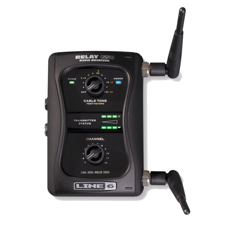
\includegraphics[width=\linewidth]{files/Receiver.png}
%    \end{subfigure}
%    \begin{subfigure}{0.4\linewidth}
%        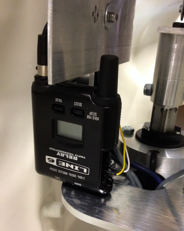
\includegraphics[width=\linewidth]{files/Transmitter.png}
%    \end{subfigure}
%    \caption{Wireless audio receiver (top) and transmitter (bottom)}
%    \label{fig:audio}
%\end{figure}

A conventional speaker is fixed on the robot and operated via the same soundcard. 
\subsection{Robot}

\begin{figure}[H]
    \centering
    \begin{subfigure}{0.3\linewidth}
        \centering
        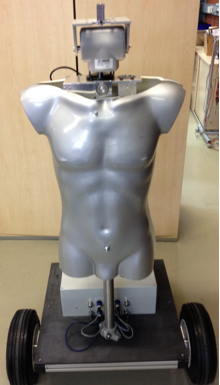
\includegraphics[height=0.3\textheight]{files/Robot.png}
        \caption{Robot designed by Gigatec S.A.}
        \label{fig:robot}
    \end{subfigure}
    \hspace{0.5em}
    \begin{subfigure}{0.3\linewidth}
        \centering
        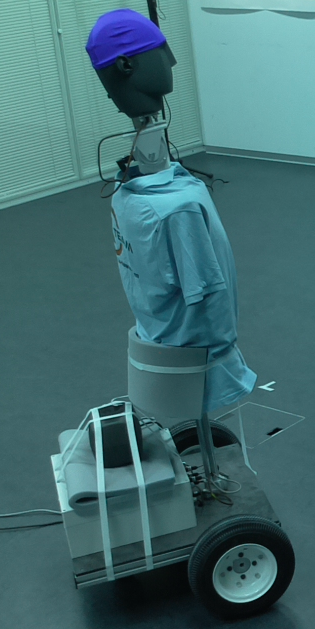
\includegraphics[height=0.3\textheight]{files/Robot2.png}
        \caption{Robot in action with acoustic head and speaker.}
        \label{fig:robot_action}
    \end{subfigure}
    \hspace{0.5em}
    \begin{subfigure}{0.3\linewidth}
        \centering
        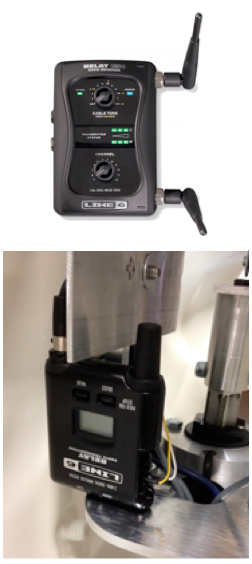
\includegraphics[height=0.3\textheight]{files/Wireless.png}
        \caption{Wireless audio receiver (top) and transmitter (bottom).}
        \label{fig:audio}
    \end{subfigure}
    \caption{Robot designed by Gigatec S.A. for Echo SLAM with wireless audio equipment and speaker.}
\end{figure}

The robot used for the experiments was designed by Gigatec S.A. It is shown in Figures \ref{fig:robot} and \ref{fig:robot_action}.
Two wheels can be actuated for displacement (see § \ref{sec:movement}) and the acoustic head can be rolled, pitched and yawed independently. 
For the present setup, the head always stays in the standard (straight) position.

For good autonomy, the robot is actuated via a socket interface and the AF\_INET protocol. All commands are sent via a \textit{python} script. For manual operation of the robot, some commands can also be sent via ssh.
%picture quality and compression:
%\url{www.raspberrypi.org/forum/viewtopic.php?f=43&t=73174&p=527300#p527300}
%wget:
%\url{https://www.maketecheasier.com/test-internet-connection-speed-from-terminal/}
%speedtest:
%http://www.speedtest.net/
